\subsection{Системы небесных координат}
Каждая из систем небесных координат является такой сферической системой координат, в которой радиус не имеет значения, так как параллакс не учитывается и звёзды считаются бесконечно удалёнными от наблюдателя.

\term{Горизонтальная система координат}~--- система координат, в которой основной плоскостью является плоскость математического горизонта, а полюсами~--- зенит и надир~--- точки небесной сферы, расположенные ровно над наблюдателем (зенит) и под ним (надир). Одной координатой является либо \imp{высота} светила $h$ (угловое расстояние между светилом и математическим горизонтом, отсчитываемое в сторону зенита), либо его \imp{зенитное расстояние} $z$ (угловое расстояние между зенитом и светилом). Другой координатой является \imp{астрономический азимут} $A$~--- угол между направлением на юг и направлением на объект, отсчитываемый в сторону запада. $NESW$~--- плоскость математического горизонта, $ZS_*Z'$~--- плоскость суточного движения светила.


\begin{figure}[!h]
\centering
	\begin{subfigure}{0.49\textwidth}
		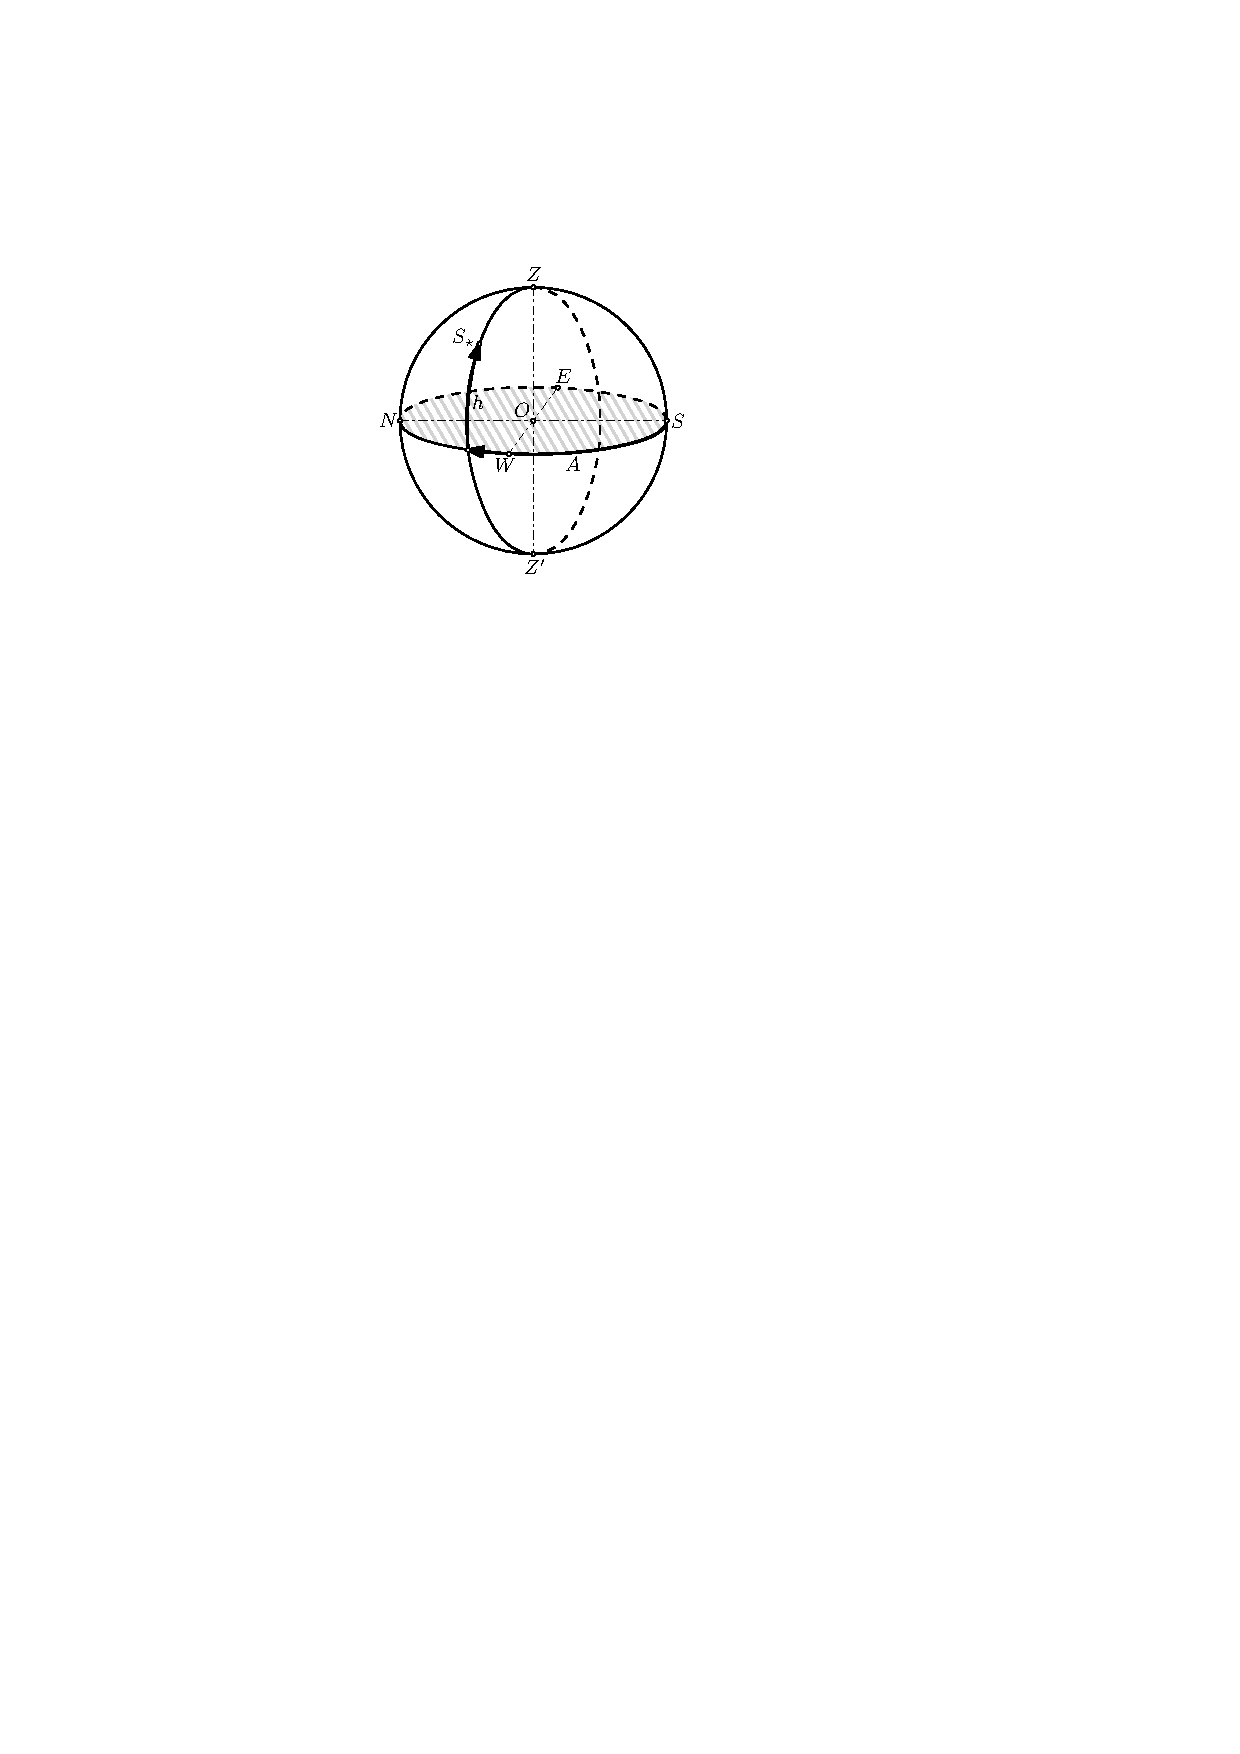
\includegraphics[width = \textwidth]{hor-coordin-sys}
		\caption{Горизонтальная система координат}
	 \end{subfigure}
	 \hfill
	\begin{subfigure}{0.49\textwidth}
		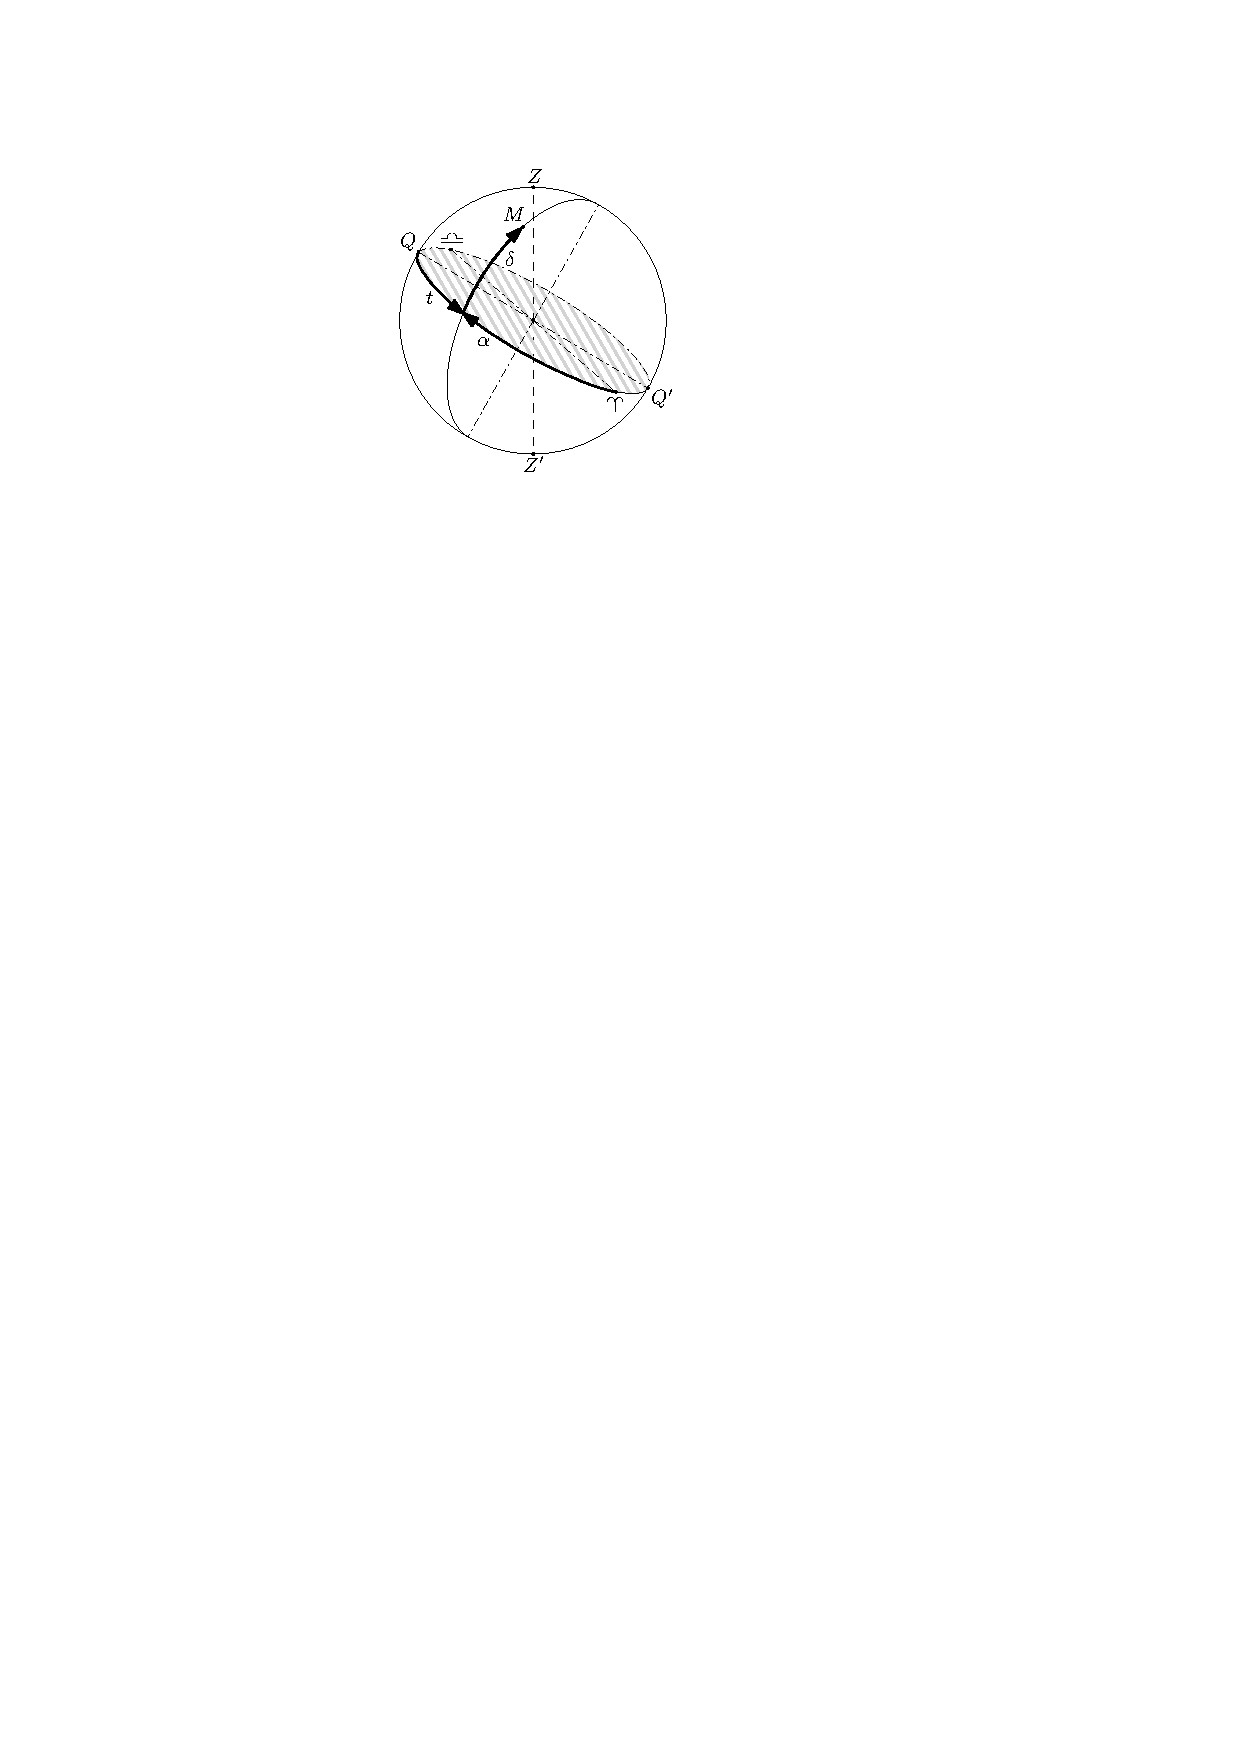
\includegraphics[width = \textwidth]{eq-coordin-sys}
		\caption{Экваториальная система координат}
	 \end{subfigure}
	\caption{Системы координат I}
\end{figure}

\term{Первая экваториальная система координат}~--- система координат, основной плоскостью которой является плоскость небесного экватора $QQ'$. Одной координатой при этом является \imp{склонение} $\delta$~--- угловое расстояние между светилом и плоскостью небесного экватора, отсчитываемое в сторону севера. Иногда вместо склонения используют \imp{полярное расстояние $p$}~--- угловое расстояние между светилом и точкой севера. Другой координатой~--- \term{часовой угол} $t$~--- дуга небесного экватора от верхней точки небесного экватора до круга склонения светила, или двугранный угол между плоскостями небесного меридиана и круга склонения светила. $\aries$ и $\libra$~--- точки весеннего и осеннего равноденствия соответственно. $P_NP_S$~--- ось мира.

\term{Вторая экваториальная система координат}~--- система, основной плоскостью которой является плоскость небесного экватора $QQ'$. Одна координата~--- \imp{склонение} $\delta$. Другой координатой является \imp{прямое восхождение} $\alpha$~--- угловое расстояние между точкой весеннего равноденствия и кругом склонения светила.


\term{Эклиптическая система координат}~--- система координат, основной плоскостью которой является плоскость эклиптики $EE'$. Одной координатой при этом является \imp{эклиптическая широта} $\beta$ (угловое растояние между светилом и эклиптикой, отсчитываемое в сторону северного полюса мира), а другой~--- \imp{эклиптическая долгота} $\lambda$ (угловое расстояние между точкой весеннего равноденствия и кругом эклиптической широты светила).

\begin{figure}[!h]

\centering
	\begin{subfigure}{0.49\textwidth}
		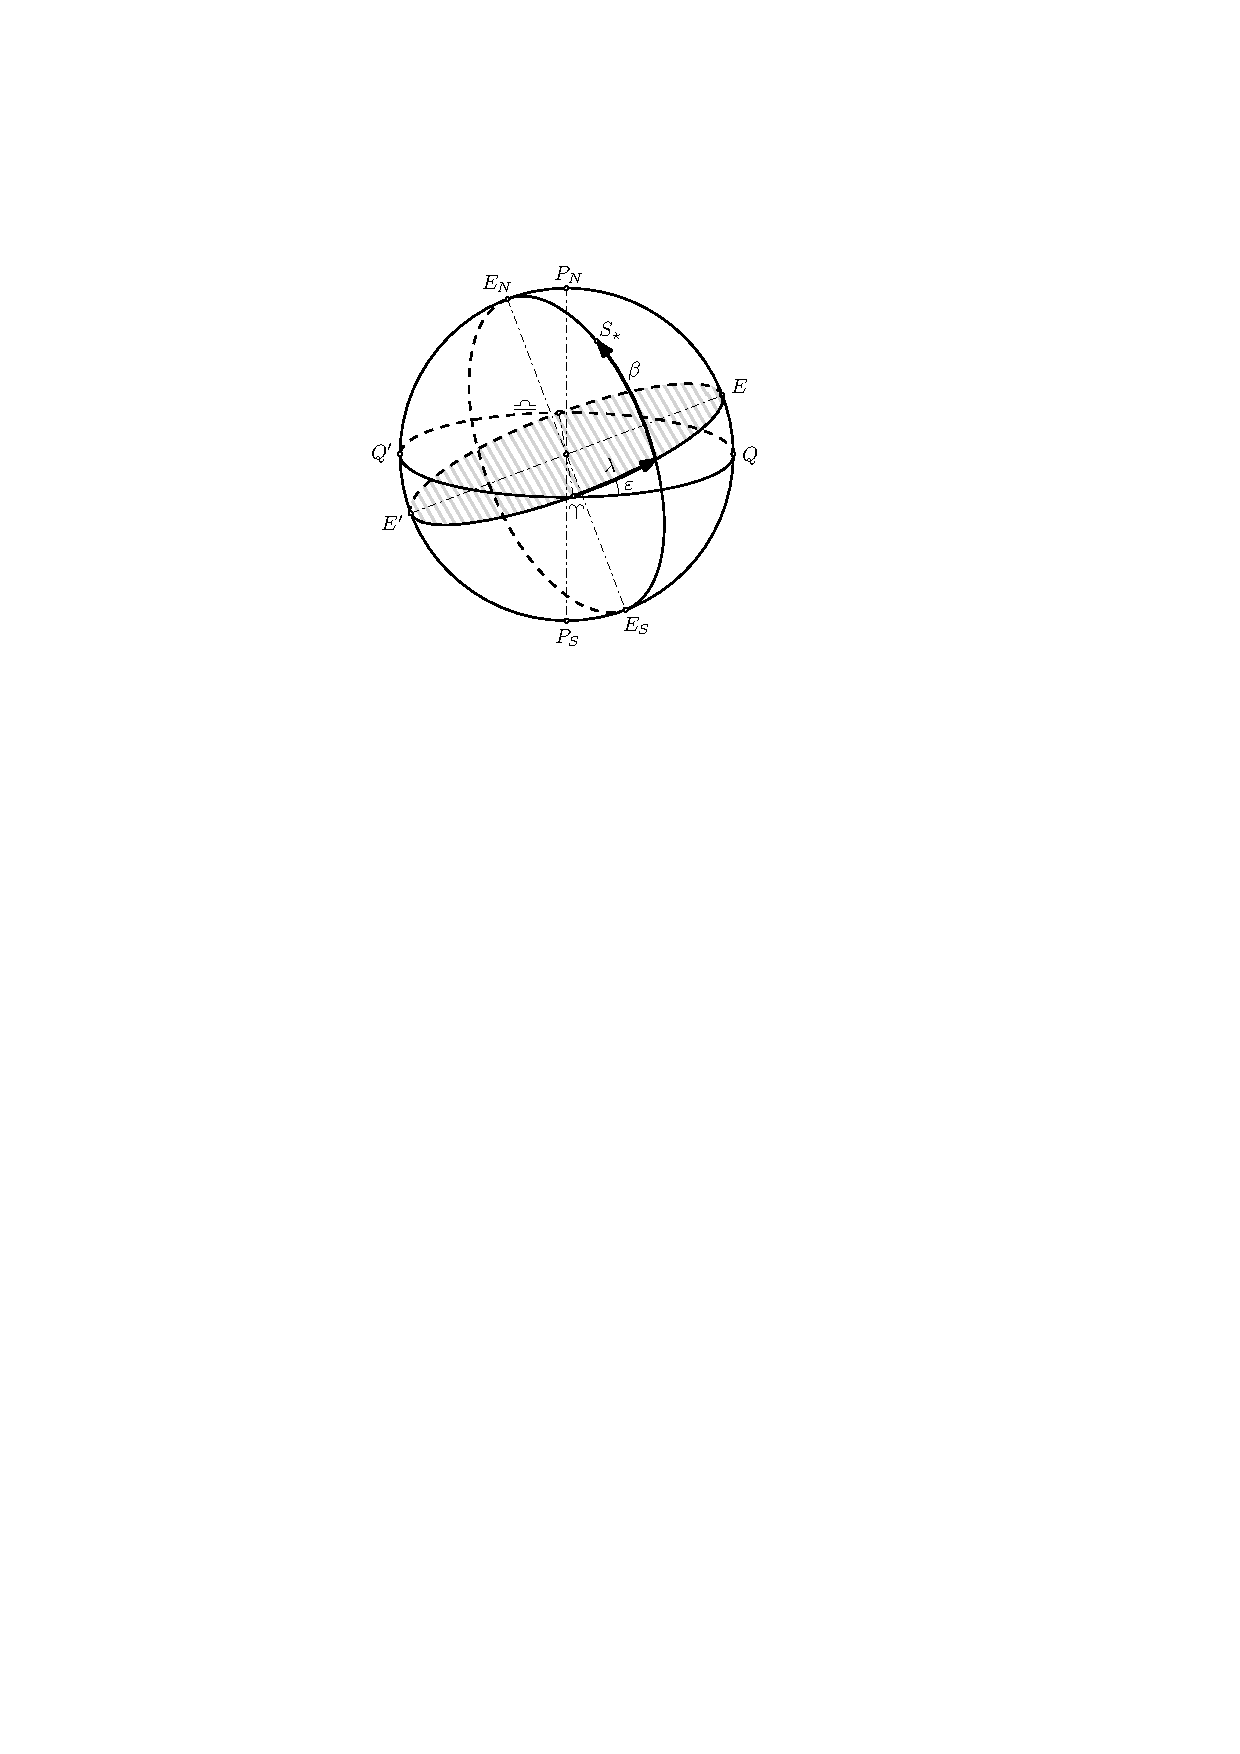
\includegraphics[width = \textwidth]{eql-coordin-sys}
		\caption{Эклиптическая система координат}
	 \end{subfigure}
	 \hfill
	\begin{subfigure}{0.49\textwidth}
		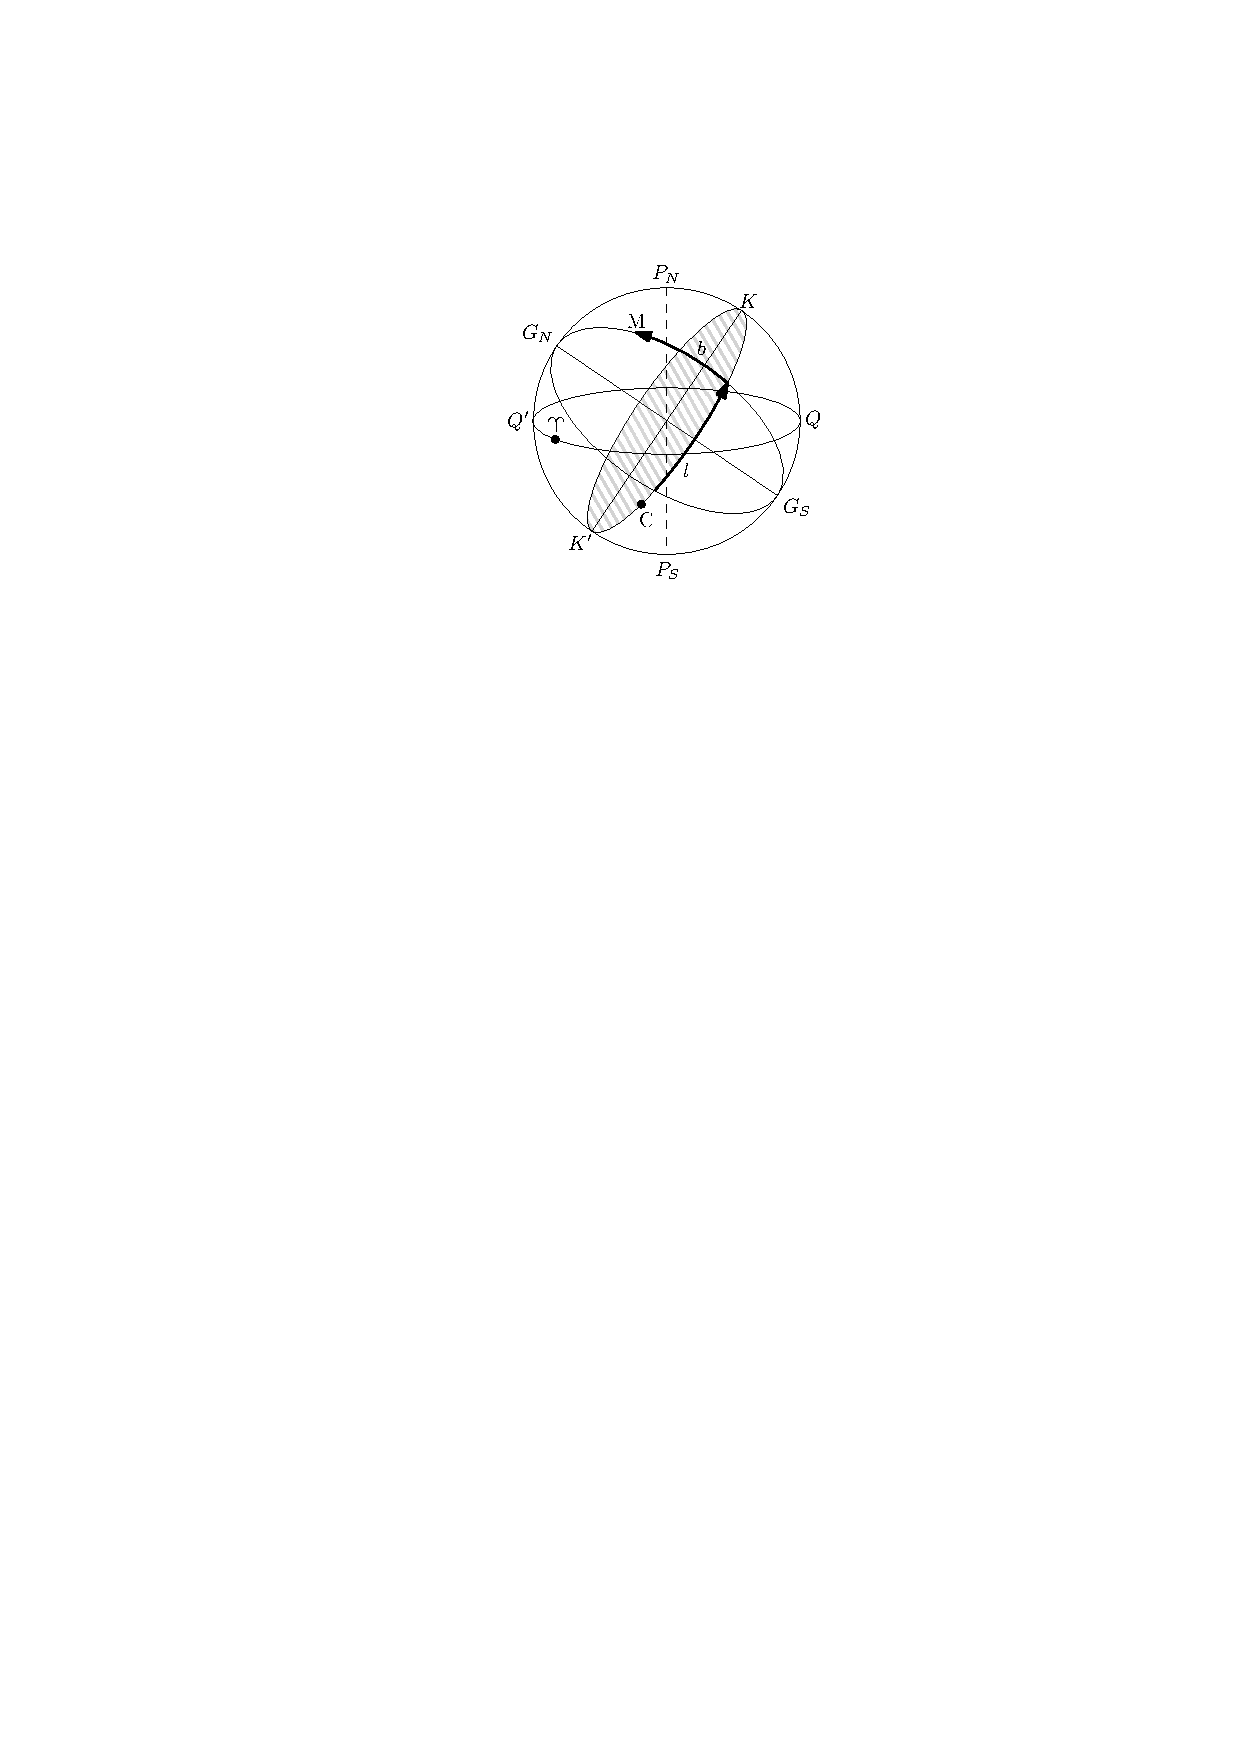
\includegraphics[width = \textwidth]{gal-coordin-sys}
		\caption{Галактическая система координат II}
	 \end{subfigure}
	\caption{Системы координат II}
\end{figure}

\term{Галактическая система координат}~--- система координат основной плоскостью которой является плоскость нашей Галактики, которая наклонена к плоскости экватора под углом $62.6^{\circ}$. Одной координатой при этом является \term{галактическая широта} $b$~--- дуга круга галактической широты от эклиптики до светила, или угол между плоскостью галактического экватора и направлением на светило, а другой~--- \term{галактическая долгота} $l$~--- дуга галактического экватора от точки начала отсчёта $C$ до круга галактической широты светила, или угол между направлением на точку начала отсчёта $C$ и плоскостью круга галактической широты светила. Точка $C$ примерно совпадает с направлением на центр галактики и имеет координаты: $\alpha=17^h45.6^m$; $\delta=-28^{\circ}56.2'$ $G_CKK'$~--- плоскость галактического экватора, $G_N$,$G_S$~--- северный и южный полюс галактики.